\documentclass{article}
\usepackage{graphicx}
\usepackage{amsmath}
\usepackage{mathrsfs}
\usepackage{amssymb} % for "\mathbb" macro
\usepackage[round]{natbib}
\usepackage{url}
\usepackage{hyperref}
\usepackage[toc,page]{appendix}

\title{Three Factor Seasonal Commodity Price Process}
\author{Jake C. Fowler}
\date{December 2020}

\begin{document}
\newcommand{\+}[1]{\ensuremath{\mathbf{#1}}}

\maketitle

WARNING: THIS DOCUMENT IS CURRENTLY WORK IN PROGRESS

\tableofcontents

\newpage

\section{Introduction}
This paper presents a specific set for parameters for the multi-factor model presented in \cite{Fowler}
such that the model should have similar statistical properties to the three-factor spot price
model presented in \cite{Boogert} the model used in the commercial KyStore gas storage valuation model. 


\section{Forward Price SDE}
The starting point is the SDE (stochastic differential equation) for the forward
price process:

\begin{align}
    \label{eq:general_forward_sde}
    \frac{dF(t, T)^l}{F(t, T)^l}=\sum_{i=1}^{n^l} \sigma_i^l(T)e^{-\alpha_i^l(T-t)}dz_i^l(t) \\
    \nonumber
    \alpha_i^l \in \mathbb{R}_{\ge 0} \\
    \nonumber
    t \in \mathbb{R}_{\ge 0} \\
    \nonumber
    T \in \{ T_0^l, T_1^l, T_2^l, \hdots | T_j^l \ge t  \} \\
    \nonumber
    \sigma_i^l : \mathbb{R}_{\ge 0} \rightarrow \mathbb{R} \\
    \nonumber
    l \in [1, m]
\end{align}

Where $z_i^l(t)$ follow correlated Wiener processes with correlation $\rho_{i, j}^{x, y}$, i.e.

\begin{equation}
    \mathbb{E}[dz_i^x(t)dz_j^y(t)] = \rho_{i, j}^{x, y}dt
\end{equation}

$F(t, T_j)^l$ is the forward price observed at time $t$, for delivery over the time 
interval $[T_j, T_{j+1})$ of the $l^{\text{th}}$ of $m$ commodity underlyings.

\section{Three Factor Seasonal Form}
The three factor seasonal parameters clearly has parameter $n=3$. The first factor is
the spot or short-term factor. For this factor there is a constant volatity and mean
reversion, i.e. $\sigma_1(T) = \sigma_{spot}$ and as this is the only factor with
non-zero mean reversion $\alpha_1 = \alpha$. This factor has the heuristic interpretation
as random shocks which move the forward curve in an exponentially decaying (as function of
time to maturity) manner, with the biggest effect being on the spot price. It can also % TODO reference clewlow strickland for SDE of spot price
be interpreted as driving random shocks to the spot price which then mean revert.

As mentioned above the remaining two factors have zero mean reversion, i.e. 
$\alpha_2 = \alpha_3 = 0$. TODO seasonal factor 

The third factor, the long-term factor, has constant volatility, $\sigma_2 = \sigma_{long}$,
and represents parallel movement which effect the whole forward curve in a maturity 
independent manner.

Finally, it is assumed that the three Brownian Motions are independent. Putting this 
together, and using the subscripts $spot$, $seas$ and $long$ the Brownian Motions
of the spot, seasonal, and long-term factors we get the following.

\begin{equation}
    \label{eq:3f_forward_sde}
    \frac{dF(t, T)}{F(t, T)}= \sigma_{spot} e^{-\alpha(T - t)} dz_{spot}(t) + \\
        \sigma_{seas}(T) dz_{seas}(t) + \sigma_{long} dz_{long}(t)
\end{equation}

Refer back to \cite{Fowler} for the statistical properties of the forward and spot
price assumed by just substituting the parameters in \cite{Fowler} with the specific
one given above.

\section{Calibration to Historical Data}
The basic ideas around calibration to historical data are givin in page 9 of \cite{Boogert}
and \cite{deJong}. The model implies the following about the dynamics of the spot and forward
prices:
\begin{itemize}
    \item $\sigma_{long}$ should approximately equals the volatility (annualised standard 
    deviation) of the log returns of an annual forward contract at the far end of the 
    forward curve. The seasonal factor will not have any net effect on annual forward 
    contract prices due to summer and winter moves cancelling each other out. The effect
    of $\sigma_{short}$ will be minimal due to the exponential decay of it's effect as
    shown in \ref{eq:3f_forward_sde}.
    \item TODO: complete this
\end{itemize}

\section{Critique of Three Factor Seasonal Model}
\subsection{Strengths of Model}

The strength of the three-factor seasonal model is it's parsimony. 
Being able to specify the gas price dynamics using only four parameters is of great help
in allowing users to intuitively see what is driving the extrinsic value of gas storage
being valued. Traders can easily adjust the input
parameters based on their view of the market. For example if a trader take a view that 
the future summer-winter spread volatility is going to be higher than in the historical
period used to calibrate the parameters they can easily bump up the seasonal volatility
parameter when valuing a potential storage deal. For a non-parsimonious model with many parameters
some of which are completely abstract (for example correlation between factors), such
usage would not be practical.

Another example of the is that risk managers can 
create scenario matrices containing storage facility (or portfolio) P\&L based on scenarios 
applied to any of the four parameters. 

% Quote Taleb and compare to Black-Scholes as a parameterisation?

It also allows for a relatively simple and intuitive way of calibrating
model parameters from historic spot and forward prices. This is of particular importance
for gas storage where there is generally a lack of liquid traded instruments which can be used
to calibrate model volatility and correlation parameters to
\footnote[1]{For many natural gas markets, there are European options traded, for which the
implied volatility can be used to calibrate price dynamics. However, the extrinsic value
of storage is mostly derived from the relative movement of different delivery points
on the forward curve, i.e. by calendar spreads. The European option volatility curve
does convey some information about calendar spread volatility (e.g. a big difference
in implied vol for two forward contracts implies that one contract will move by much
more than another, hence higher calendar spread volatility) but not enough to fully 
calibrate the joint price dynamics of the whole forward curve.}.

% TODO cite other Kyos paper
The KyStore product is clearly a popular one and The Author believes that this is at least partially due 
to the parsimony of the underlying price process model.

\subsection{Weaknesses of Model}
The big downside of this model is that the forward volatility seasonality structure is unrealistic.
It is well known that, adjusting for time-to-maturity effects, the volatility of winter periods 
will generally be higher than those in summer. Figure \ref{fig:seasonal_vol} plots the forward
volatility implied by the model, with mean reversion set to zero in order to remove any t
time-to-maturity effect. This chart shows that the model implies two volatility peaks a
year, once in February, as expected, but the other around August.
Although the three factor seasonal model captures summer versus winter seasonality, it 
does not capture the higher frequency day-of-week seasonality. With day-of-week 
seasonality a lower correlation of returns would be expected between weekday and weekend 
foward delivery dates, than between pairs of days which are both weekdays or weekend days
respectively. This is after taking into account non-seasonal reduced correlation due to the 
difference in delivery dates. Such day-of-week seasonality would likely % TODO reference Rebonator
have an impact on fast storage where some cycling of volume might be optimal across
the weekend-weekday boundary. It is unlikely to have any effect on slow storage.

\section{Future Work}
% \subsection{Addressing Model Weaknesses}
This section describes briefly potential future which could be done to extend the three
factor model in order to address the weaknesses presented above.
% TODO better summer-winter seasonal 
Decorrelation between weekdays weekend days could be achieved by adding a fourth factor.
% TODO examples of factors
However, one problem with adding a fourth weekday-weekend factor is calibration. Often
there will not be forward market prices for individual days beyond day-ahead which makes
the correlation between weekdays and weekend days something which can't be observed.
Another problem is that the addition of a fourth factor will diminish the models
parsimony. Some experimentation on whether decorrelating weekdays and weekends
has any material impact on the valuation of storage facilities of interest should be
conducted as a consideration to whether it is worth adding the extra factor.

% TODO calibration using integrated covariances instead

\begin{figure}
    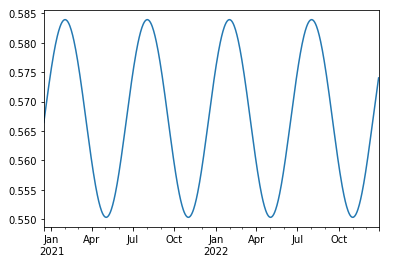
\includegraphics{vol_seasonality.png}
    \caption{Forward Volatility By Delivery Date}
    \label{fig:seasonal_vol}
\end{figure}


\bibliographystyle{plainnat}
\bibliography{three_factor_seasonal_model}

\end{document}